% ==============================================================================
% SECCION 2: ACTIVIDAD 1 - NAND3 DINAMICA FOOTED
% ==============================================================================
\needspace{6\baselineskip}
\section{Actividad 1: NAND3 CMOS Dinámica Footed (Fases, Asimetría y Consumo)}
\label{sec:actividad1}

\subsection{Topología Circuital y Dimensionamiento}
La compuerta NAND3 dinámica analizada se implementa en configuración \textit{footed} complementada por un inversor dominó restaurador, operando bajo tecnología PTM de 45\,nm HP ($V_{DD} = 1.0\,\text{V}$, $T = 27^\circ\text{C}$). 

\begin{itemize}[leftmargin=1.4em,itemsep=0.15em]
  \item \textbf{Red de Descarga (PDN) y Footer ($M_f$):} Cuatro transistores NMOS en serie ($M_1, M_2, M_3$ para las entradas lógicas $A, B, C$, y $M_f$ para $CLK$). Los tres NMOS lógicos y el footer adoptan $W_n = 3 \times 90\,\text{nm} = 270\,\text{nm}$ ($L = 45\,\text{nm}$); la aproximación geométrica de cuatro dispositivos en serie establece una anchura efectiva de $W_{PDN,eq} = 270\,\text{nm}/4 = 67.5\,\text{nm}$ (consistente con el modelado de contención en la Actividad~3), en lugar de equiparar exactamente a un NMOS unitario de $90\,\text{nm}$.
  \item \textbf{Transistor de Precarga ($M_p$):} Dispositivo PMOS ($W_p = 135\,\text{nm}$, $L = 45\,\text{nm}$) conectado a $V_{DD}$, gobernado por $CLK$ en nivel bajo ($\beta = 1.5$ respecto al NMOS de $90\,\text{nm}$).
  \item \textbf{Inversor Dominó de Salida:} Etapa restauradora no inversora con $M_{pi}$ ($W_p = 135\,\text{nm}$) y $M_{ni}$ ($W_n = 90\,\text{nm}$).
  \item \textbf{Condiciones de Carga:} Capacitancia concentrada explícita $C_L = 2\,\text{fF}$ en el nodo interno $dyn$ y capacitancia de carga $C_{out} = 1\,\text{fF}$ en el terminal de salida $out$.
  \item \textbf{NAND3 CMOS Estática Equivalente:} PUN de 3 PMOS en paralelo ($W_p = 135\,\text{nm}$) y PDN de 3 NMOS en serie ($W_n = 270\,\text{nm}$), con carga idéntica $C_{out} = 1\,\text{fF}$.
\end{itemize}

Estructuralmente, el núcleo dinámico \textit{footed} requiere únicamente 5 transistores (4 NMOS + 1 PMOS) y 7 transistores con la etapa dominó completa, frente a los 6 transistores requeridos por la NAND3 estática convencional.

\subsection{Análisis Temporal y Fases de Operación}
Para caracterizar el ciclo secuencial, se aplicó reloj a $500\,\text{MHz}$ ($T_{clk} = 2.0\,\text{ns}$, ciclo de trabajo del 50\%) y un estímulo de entrada $A$ a $125\,\text{MHz}$ ($T_A = 8.0\,\text{ns}$) con retardo de $t_{\text{delay}} = 1.1\,\text{ns}$ ($0.55\,T_{clk}$), fijando $B=C=V_{DD}$. Las curvas se ilustran en la Figura~\ref{fig:fases_formas_onda}, distinguiéndose las cuatro fases operativas:

\begin{figure}[htbp]
  \centering
  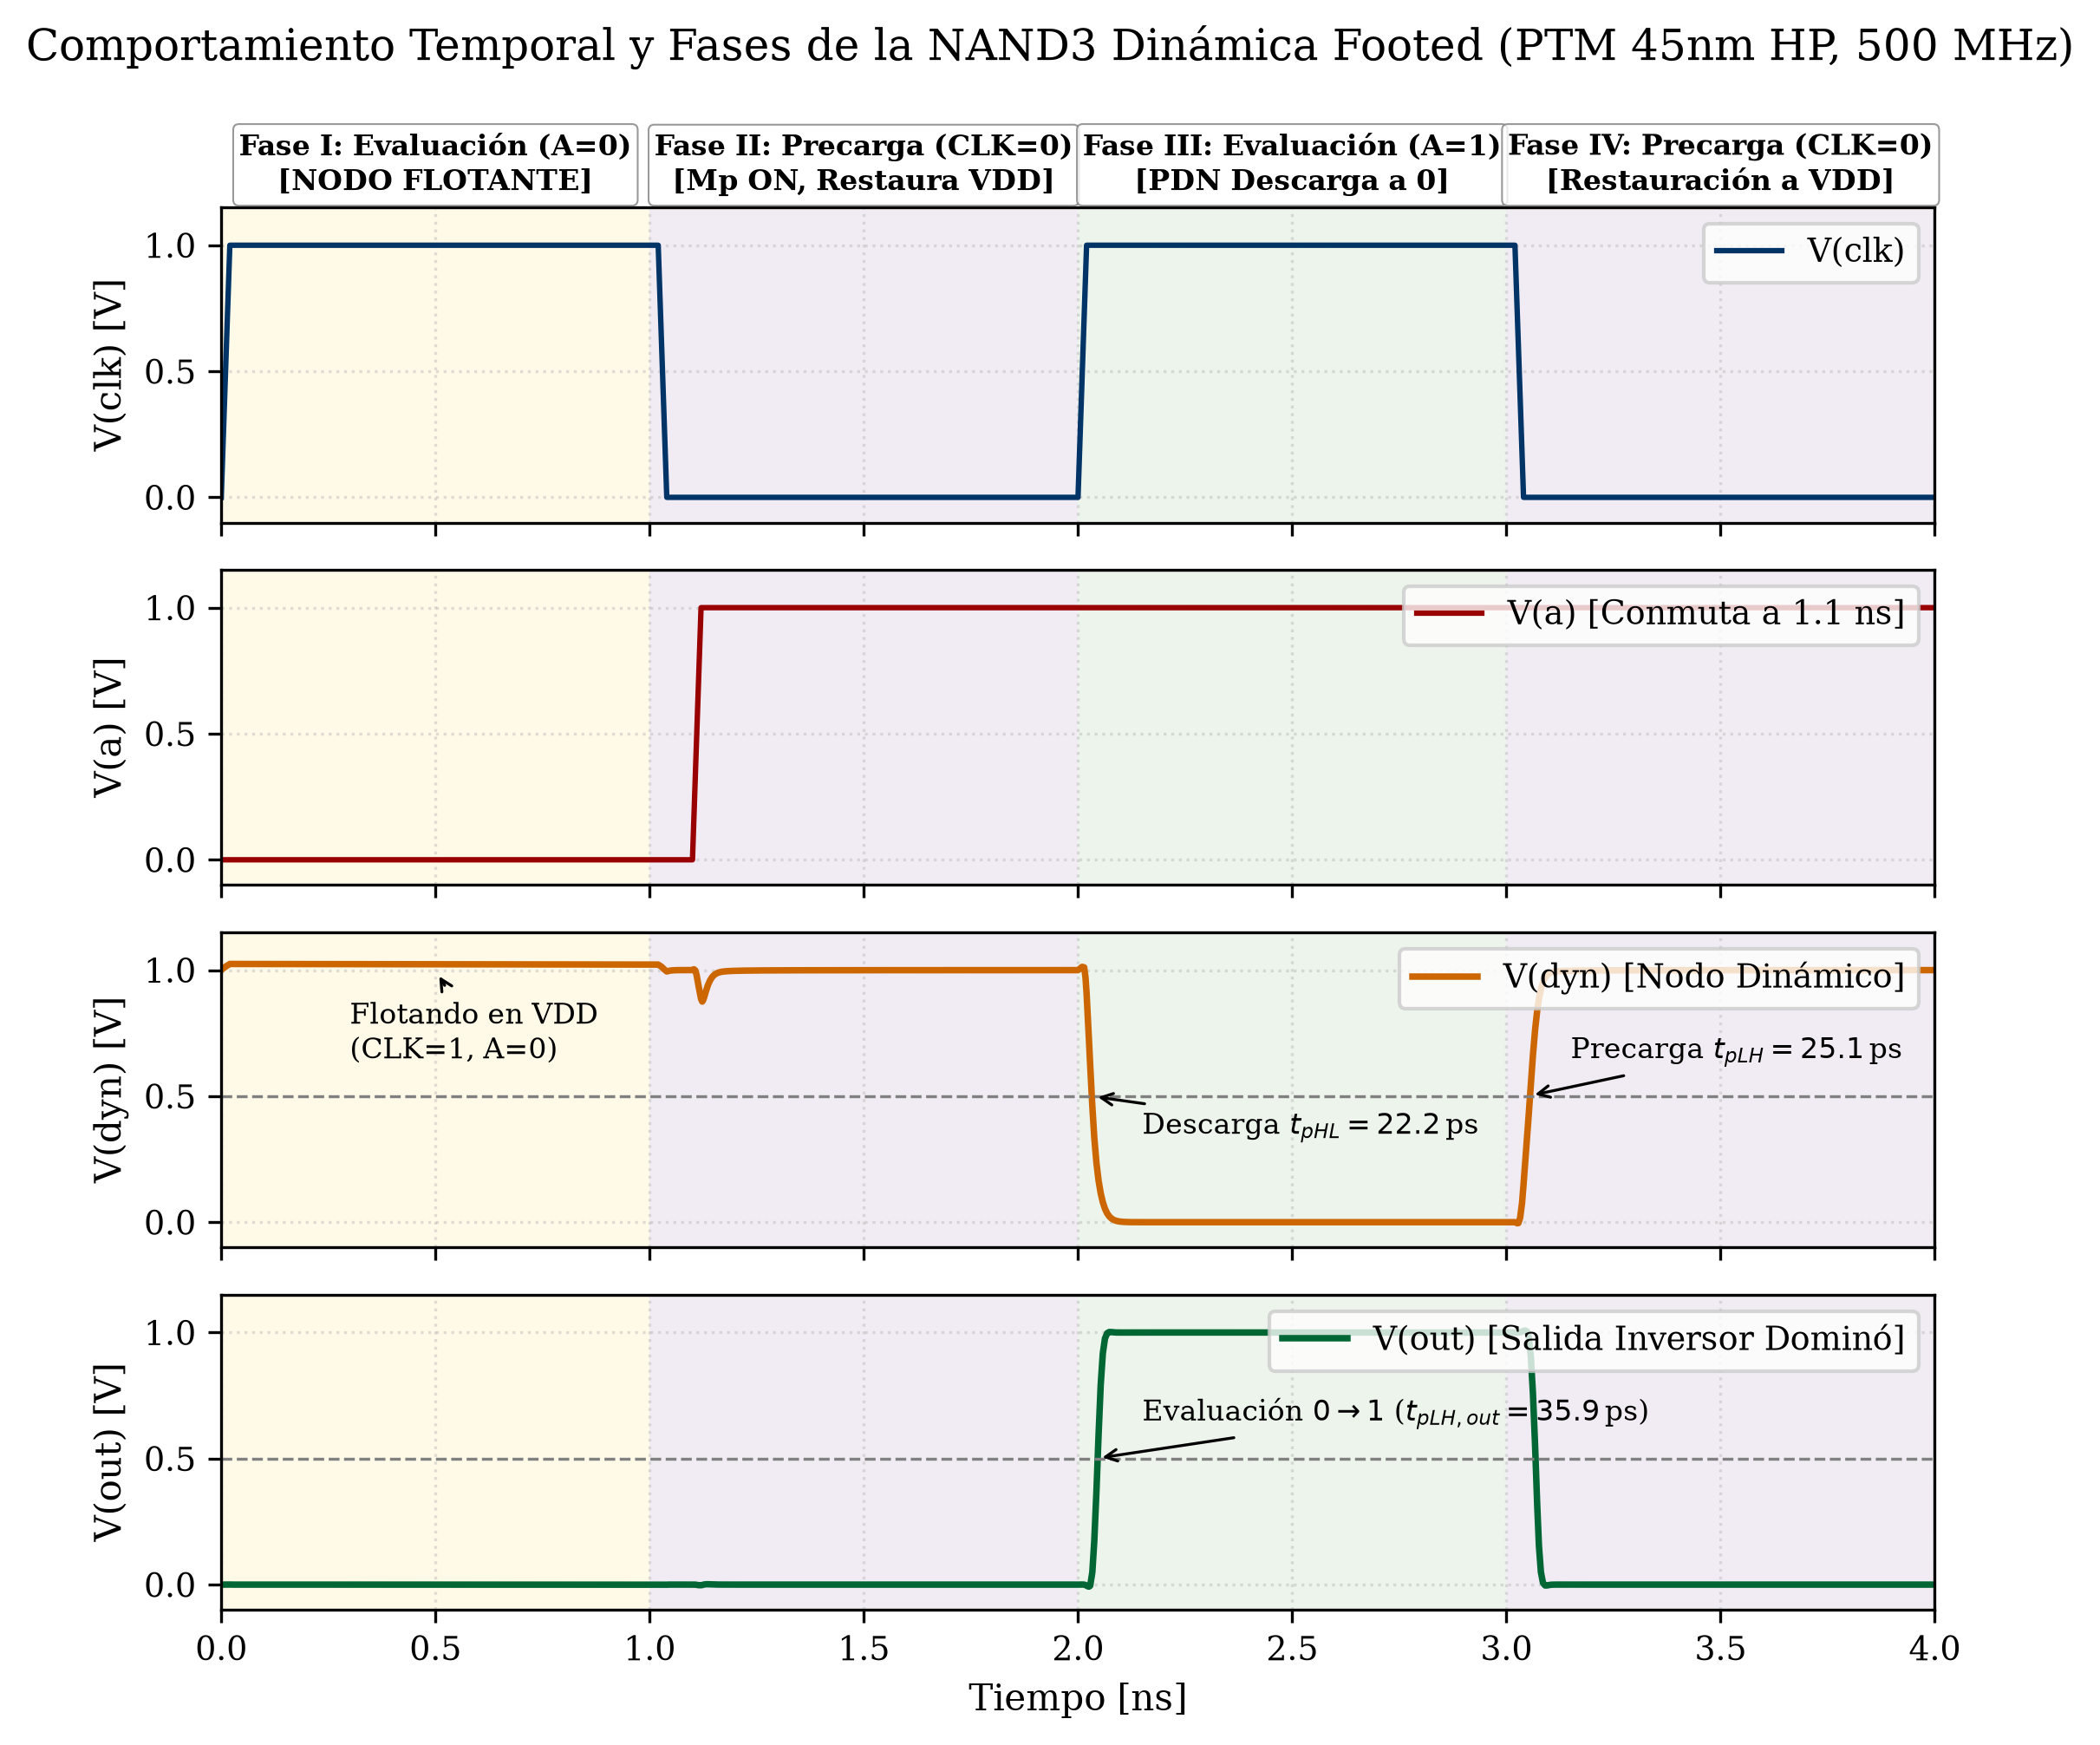
\includegraphics[width=0.44\linewidth]{figuras/fig1_act1_fases_formas_onda.png}
  \caption[Formas de onda transitorias de la NAND3 dinámica footed]{Formas de onda transitorias de la NAND3 dinámica footed ($CLK$, $A$, nodo interno $dyn$ y salida $out$), identificando las cuatro fases de operación dominó.}
  \label{fig:fases_formas_onda}
\end{figure}

\begin{enumerate}[leftmargin=1.4em,itemsep=0.12em]
  \item \textbf{Fase I: Evaluación con PDN Abierta ($t \in [0.0,\, 1.0\,\text{ns}]$):} Con $CLK = 1$, $M_p$ corta y $M_f$ conduce. Al estar $A = 0$, $M_1$ bloquea la ruta a tierra; el nodo $dyn$ queda \textbf{flotante en nivel alto} ($V_{DD} = 1.0\,\text{V}$) con un sobreimpulso a $1.022\,\text{V}$ por acoplamiento capacitivo (\textit{clock feedthrough} en $C_{gd}(M_p)$). La salida $out$ permanece en $0\,\text{V}$.
  \item \textbf{Fase II: Precarga con $A=1$ ($t \in [1.0,\, 2.0\,\text{ns}]$):} Con $CLK = 0$, $M_p$ conduce y $M_f$ corta. Aunque $A$ conmuta a 1 en $t = 1.1\,\text{ns}$, el footer apagado impide el paso a tierra. El nodo $dyn$ se mantiene rígidamente fijado a $V_{DD}$.
  \item \textbf{Fase III: Evaluación con Descarga Completa ($t \in [2.0,\, 3.0\,\text{ns}]$):} Con $CLK=1$ y $A=B=C=1$, los 4 NMOS conducen. El nodo $dyn$ se descarga a tierra en $t_{pHL,dyn} = 22.17\,\text{ps}$, haciendo que el inversor dominó conmute monótonamente en su salida $out$ con $t_{pd,\text{eval}} = 35.89\,\text{ps}$.
  \item \textbf{Fase IV: Precarga y Restauración ($t \in [3.0,\, 4.0\,\text{ns}]$):} En el flanco descendente de $CLK$, $M_p$ recarga el nodo $dyn$ en $t_{pLH,dyn} = 25.13\,\text{ps}$, restaurando la salida $out$ a nivel bajo en $t_{pHL,out} = 38.06\,\text{ps}$.
\end{enumerate}

\subsection{Asimetría Temporal y Rol de \texorpdfstring{$t_{pLH}$}{tpLH} en Lógica Dominó}
En lógica dominó, el cómputo combinacional ocurre exclusivamente durante la evaluación ($CLK = 1$), con salidas conmutando monótonamente ($0 \to 1$). El tiempo de precarga medido en el nodo dinámico ($t_{pLH,dyn} = 25.13\,\text{ps}$) corresponde estrictamente al retardo de transición al 50\% ($CLK\downarrow$ al 50\% hasta $dyn\uparrow$ al 50\%) durante el semi-periodo inactivo ($CLK = 0$), fuera de la ruta crítica de datos; por consiguiente, \textbf{no contribuye al retardo lógico de evaluación}.

Es metodológicamente necesario precisar que dicho retardo al 50\% no debe equipararse directamente al tiempo de asentamiento casi completo del nodo ($V_{dyn} \ge 0.99\,V_{DD}$). Como referencia analítica, en un circuito $RC$ ideal inicialmente descargado ($V(t) = V_{DD}(1 - e^{-t/\tau_{\text{pre}}})$), el tiempo requerido para alcanzar el 99\% de $V_{DD}$ es $t_{99} = -\tau_{\text{pre}} \ln(0.01) \approx 4.605\,\tau_{\text{pre}}$ (mientras que $3\,\tau_{\text{pre}}$ restaura el 95.0\% y $4\,\tau_{\text{pre}}$ el 98.2\%). Aunque la compuerta dinámica real involucra la respuesta no lineal del PMOS de precarga ($M_p$ de saturación a triodo), esta referencia analítica justifica que el semi-periodo bajo de reloj deba satisfacer holgadamente $T_{clk}/2 \ge t_{\text{precarga}}$ para garantizar restauración plena.

\subsection{Comparación Cuantitativa: Lógica Dinámica vs Estática}
La Tabla~\ref{tab:comparativa_act1} resume las métricas cuantitativas extraídas, contrastando la estructura dinámica con la estática equivalente.

% Tabla generada automaticamente por generar_tablas_latex.py
% Fuente de datos: act1_metricas.json (Trazabilidad 100% verificada)
\begin{table}[htbp]
\centering
\scriptsize
\setlength{\tabcolsep}{3.5pt}
\caption[Comparación cuantitativa entre NAND3 dinámica footed y CMOS estática]{Comparación cuantitativa entre la compuerta NAND3 dinámica footed (con inversor dominó) y la NAND3 CMOS estática (PTM 45\,nm HP, $V_{DD}=1.0\,\text{V}$, $T=27^\circ\text{C}$).}
\label{tab:comparativa_act1}
\begin{tabularx}{\linewidth}{@{}>{\RaggedRight\arraybackslash}p{3.2cm} c c c >{\RaggedRight\arraybackslash}X@{}}
\toprule
\textbf{Métrica Evaluada} & \textbf{NAND3 Dinámica} & \textbf{NAND3 Estática} & \textbf{Cociente} & \textbf{Condición / Notas Metodológicas} \\
\midrule
N.º de Transistores & 5 (núcleo) / 7 (total) & 6 & 0.83 / 1.17 & Topología footed + inversor dominó \\
$t_{pHL}$ (Descarga nodo $dyn$) & 22.17\,ps & 9.61\,ps & 2.306$\times$ & Evaluación $dyn$ vs caída $out\_stat$ \\
$t_{pLH}$ (Precarga nodo $dyn$) & 25.13\,ps & 12.40\,ps & 2.026$\times$ & Precarga $dyn$ vs subida $out\_stat$ \\
\midrule
\multicolumn{5}{@{}l@{}}{\textbf{Retardo en Salidas Lógicas (Triggers Asimétricos)}} \\
Retardo en terminal $out$ & 35.89\,ps ($CLK\uparrow$) & 9.61\,ps ($A\uparrow$) & 3.733$\times$ & $C_{out}=1\,\text{fF}$. Triggers distintos ($CLK\uparrow$ vs $A\uparrow$) \\
\midrule
\multicolumn{5}{@{}l@{}}{\textbf{Control con Carga Concentrada Desacoplada ($C_L=0\,\text{fF}$)}} \\
Respuesta con $C_L=0\,\text{fF}$ & $t_{pHL,dyn}=11.26\,\text{ps}$ & --- & --- & Retiene parásitas de difusión, MOS y compuerta del inversor ($M_{pi}, M_{ni}$) \\
                                    & $t_{pd,\text{eval}}=21.27\,\text{ps}$ & & & \\
\midrule
Capacitancia de Entrada $C_{in}(A)$ & 0.3417\,fF & 0.5936\,fF & 0.5756 & Reducción de 42.4\% por eliminación de PUN \\
\midrule
$P_{\text{avg}}$ ($A$ conmutando a 125\,MHz) & 1.2393\,$\mu$W & 0.2692\,$\mu$W & 4.604$\times$ & Estímulo idéntico $T_A=8\,\text{ns}$, $CLK=500\,\text{MHz}$ \\
$P_{\text{avg}}$ (Entradas fijas en nivel 1) & 2.7255\,$\mu$W & 1.7004\,nW & 1602.9$\times$ & Trampa de potencia: $\alpha=1$ ($CLK$) vs $\alpha=0$ \\
\bottomrule
\end{tabularx}
\end{table}


\begin{figure}[htbp]
  \centering
  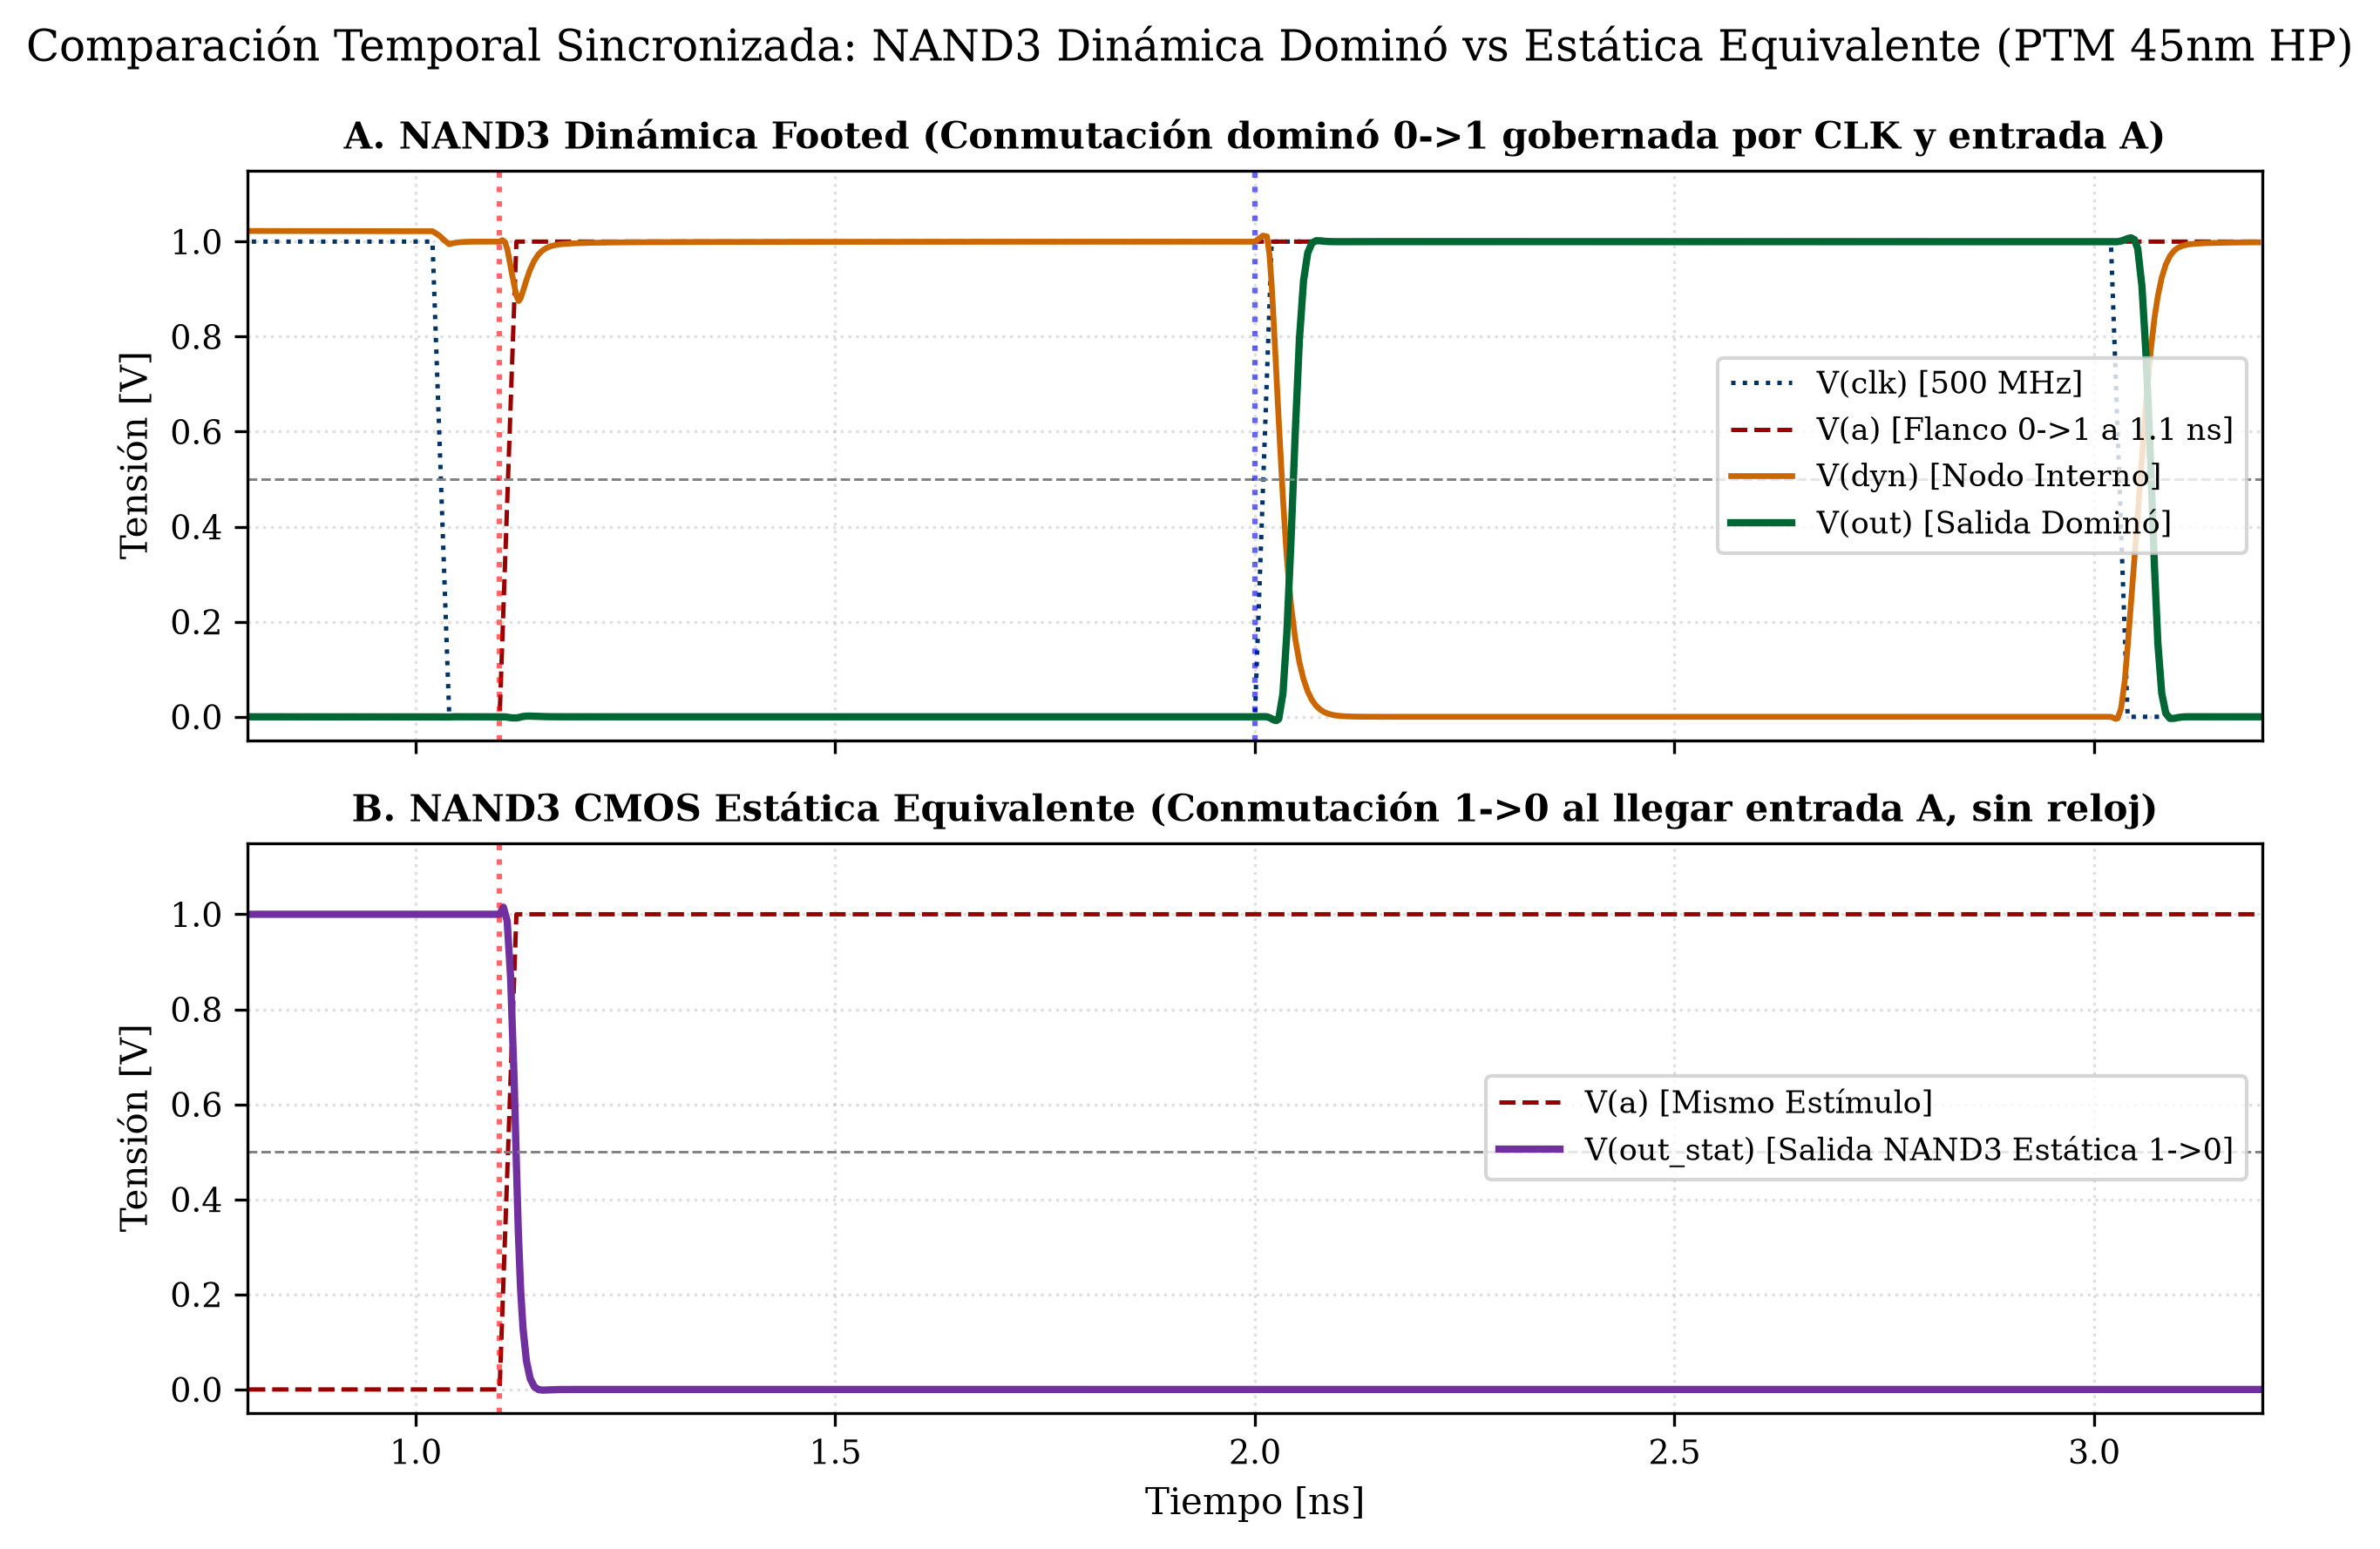
\includegraphics[width=0.42\linewidth]{figuras/fig2_act1_dinamica_vs_estatica.png}
  \caption[Comparación temporal entre NAND3 dinámica y estática]{Comparación temporal sincronizada entre la NAND3 dinámica footed y la NAND3 CMOS estática bajo el mismo estímulo de entrada $V(a)$ ($T_A=8\,\text{ns}$).}
  \label{fig:dinamica_vs_estatica}
\end{figure}

\noindent\textbf{Retardo de Evaluación y Triggers Asimétricos:} En los terminales de salida con carga nominal $C_{out} = 1\,\text{fF}$, la compuerta dominó registra un retardo de evaluación de $\mathbf{35.89\,\text{ps}}$ desde el disparo sincrónico $CLK\uparrow$ con $A=1$, mientras que la compuerta estática presenta $\mathbf{9.61\,\text{ps}}$ desde el dato asíncrono $A\uparrow$ (cociente descriptivo de $3.733\times$). Al suprimir la carga artificial concentrada (con carga concentrada desacoplada, $C_L = 0\,\text{fF}$), el retardo en $dyn$ cae a $t_{pHL,dyn} = 11.26\,\text{ps}$ y la salida conmuta en $t_{pd,\text{eval}} = 21.27\,\text{ps}$, reteniendo únicamente las capacitancias parásitas de difusión y compuerta del inversor.

\noindent\textbf{Capacitancia de Entrada ($C_{in}$):} En la caracterización dinámica de entrada, la integración de la corriente de entrada ante una rampa de $50\,\text{ps}$ ($Q_{in} = \int -I(V_a)\,dt$, $C_{in} = Q_{in}/V_{DD}$) arrojó $C_{in,\text{dyn}} = \mathbf{0.3417\,\text{fF}}$ frente a $C_{in,\text{stat}} = \mathbf{0.5936\,\text{fF}}$ en la estática, logrando una reducción del \textbf{42.4\%} ($0.5756\times$) debida a la eliminación de la red PMOS de pull-up en los datos. El modelo analítico de placas paralelas ($C_{ox,n} W_n L \approx 0.336\,\text{fF}$ y $C_{ox,n} W_n L + C_{ox,p} W_p L \approx 0.497\,\text{fF}$) concuerda con esta tendencia, reflejando la simulación en gran señal los aportes de solapamiento ($C_{ov}$) e inversión fuerte.

\subsection{Análisis de Potencia y la ``Trampa de Potencia''}
Bajo estímulo periódico en $A$ a $125\,\text{MHz}$ ($T_A=8\,\text{ns}$), la compuerta dinámica consume $P_{\text{dyn}} = 1.2393\,\mu\text{W}$ frente a $P_{\text{stat}} = 0.2692\,\mu\text{W}$ ($4.604\times$), integradas entre $4$ y $16\,\text{ns}$. Sin embargo, la manifestación crítica de la \textit{trampa de potencia} se evidencia con entradas fijas en alto ($A=B=C=1$): mientras que la compuerta estática permanece en reposo disipando únicamente fugas ($P_{\text{stat}} = \mathbf{1.7004\,\text{nW}}$ para $\alpha=0$), la compuerta dinámica cicla continuamente a $500\,\text{MHz}$ ($\alpha=1$), consumiendo $P_{\text{dyn}} = \mathbf{2.7255\,\mu\text{W}}$ (\textbf{1602.9 veces superior}). La disipación total medida de la fuente ($2.7255\,\mu\text{W}$) supera a la potencia dinámica analítica de carga externa ($P_{\text{ext}} = C_L V_{DD}^2 f = 1.000\,\mu\text{W}$) y del nodo dinámico ($P_{\text{nodo,geom}} \approx 1.325\,\mu\text{W}$ para $C_{dyn} \approx 2.65\,\text{fF}$) debido a la conmutación periódica del inversor dominó cargando $C_{out}=1\,\text{fF}$, transiciones de cortocircuito y difusiones.

\subsection{Comportamiento de Retención Preliminar con PDN Abierta}
Fijando $V_c = 0\,\text{V}$ (bloqueo en $M_3$ con $A=B=V_{DD}$), el nodo dinámico queda flotante en nivel alto. En la escala nominal ($T_{clk} = 2\,\text{ns}$, 1\,ns de evaluación), la caída por fugas es inocua: $V(dyn)_{\text{min}} = 0.9936\,\text{V}$ ($\Delta V = 6.41\,\text{mV}$, $V_{out,\text{max}} = 0.31\,\text{mV}$). Sin embargo, al extender la evaluación continua a baja frecuencia ($T_{clk} = 400\,\text{ns}$, evaluación de $200\,\text{ns}$), las corrientes de fuga subumbral drenan la carga hasta $V(dyn)_{\text{final}} = \mathbf{0.8837\,\text{V}}$ ($\Delta V = \mathbf{116.28\,\text{mV}}$). Aunque a $27^\circ\text{C}$ el potencial aún supera $V_M \approx 0.48\,\text{V}$, esta degradación evidencia la volatilidad de la carga en nodos flotantes y fundamenta la necesidad de una frecuencia mínima ($f_{\text{min}}$) y de circuitos keeper, fenómeno que se caracteriza en profundidad en la Actividad~3.

\subsection{Conclusiones de la Actividad 1}
\begin{enumerate}[leftmargin=1.4em,itemsep=0.12em]
  \item La lógica dominó reduce la capacitancia de entrada en 42.4\% ($0.3417\,\text{fF}$ vs $0.5936\,\text{fF}$), mejorando la velocidad de excitación de etapas previas.
  \item El semi-periodo de precarga no retrasa la evaluación pero su constante de tiempo acota la frecuencia máxima ($T_{clk}/2 \ge t_{\text{precarga}}$).
  \item Con entradas estáticas en nivel alto, la alternancia forzada de precarga y evaluación genera un consumo dinámico $1602.9\times$ superior al reposo estático.
  \item La pérdida de $116.28\,\text{mV}$ en $200\,\text{ns}$ con PDN abierta ratifica la naturaleza cuasi-estática de la compuerta y exige mecanismos activos de retención.
\end{enumerate}
